% Belt and pulley system
% Author: Jimi Oke
\documentclass[tikz,border=10pt]{standalone}
\usepackage{tikz}
\usetikzlibrary{arrows,shapes,positioning}
\begin{document}
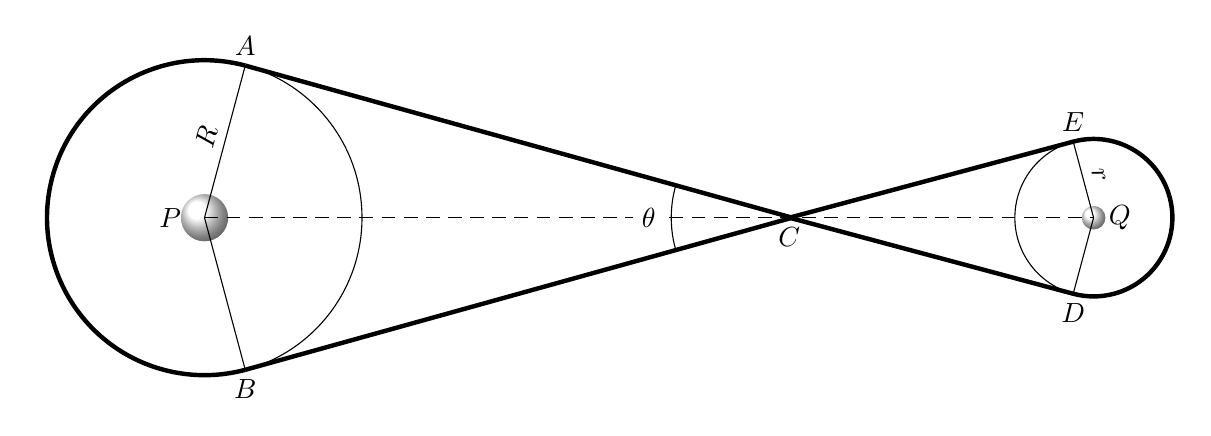
\begin{tikzpicture}
 
      % Definitions
      \pgfmathsetmacro{\b}{75}
      \pgfmathsetmacro{\a}{15}
      \pgfmathsetmacro{\R}{2}
      \pgfmathsetmacro{\r}{1}
      \pgfmathsetmacro{\P}{\R*tan(\b)}
      \pgfmathsetmacro{\Q}{\R/cos(\b)}
      \pgfmathsetmacro{\p}{\r/tan(\a)}
      \pgfmathsetmacro{\q}{\r/sin(\a)}

      % Pulleys
      
      % big pulley
      \draw (0,0) circle (\R) ;
      %\fill[left color=gray!80, right color=gray!60, middle
        color=white] (0,0) circle (\R) ;
      \draw[thick, white] (0,0) circle (.8*\R);
      \shade[ball color=white] (0,0) circle (.3) node[left,xshift=-5] {$P$};

      % small pulley
      \draw (\Q+\q-.3, 0) circle (\r);
      %\fill[left color=gray!80, right color=gray!60, middle
        color=white] (\Q+\q-.3, 0) circle (\r) ;
      \draw[thick, white] (\Q+\q-.3,0) circle (.8*\r);
      \shade[ball color=white] (\Q+\q-.3,0) circle (.15) 
      node[right, xshift=2] {$Q$};

      % belt and point labels
      \begin{scope}[ultra thick]
        \draw (\b:\R) arc (\b:360-\b:\R) ;
        \draw (\b:\R) -- ( \P, 0 ); 
        \draw (-\b:\R) -- ( \P, 0 );
        \draw (\Q-.3,0) -- + (\a:\p)  arc (105:-105:\r) ;
        \draw (\Q-.3,0) -- + (-\a:\p);
        %\draw (\b:\R) arc (\b:360-\b:\r) ;
      \end{scope}
   
      \draw (0,0) -- (\b:\R) node[midway, above,sloped] {$R$} node[above] {$A$};
      \draw (-\b:\R)--(0,0) ;
      \draw (\Q+\q-.3,0) -- +(105:\r) node[midway,above, sloped] {$r$}
        node[above] {$E$};
      \draw (\Q+\q-.3,0) -- +(-105:\r) node[below] {$D$};
      \node[below] at (-\b:\R) {$B$};
      \node[below] at (\Q-.3,0) {$C$};

      % center line
      \draw[dash pattern=on5pt off3pt] (0,0) -- (\Q+\q-.3,0);

      % angle label
      \node[fill=white] at (0.73*\Q, 0) {$\theta$} ;
      \draw (\Q-1.8,0) arc (180:195:1.5);
      \draw (\Q-1.8,0) arc (180:165:1.5);
\end{tikzpicture}
\end{document} 